\documentclass[../syllabus.tex]{subfiles}

\begin{document}

\section{Codeer Koch's Curve}
Vandaag gaan we door middel van \texttt{recursieve functies} fractals tekenen!
In de vorige \textit{assignment} heb je de functie \texttt{kochCurve} geschreven die de figuur \ref{fig:koch} tekent. Als je iedere lijn vervangt door deze zelfde figuur krijg je de situatie van figuur \ref{fig:koch2}. Als je dit oneindig vaak herhaald krijg je een \textbf{fractel} (zie figuur \ref{fig:koch_fract}).
\begin{figure}[H]
	\centering
	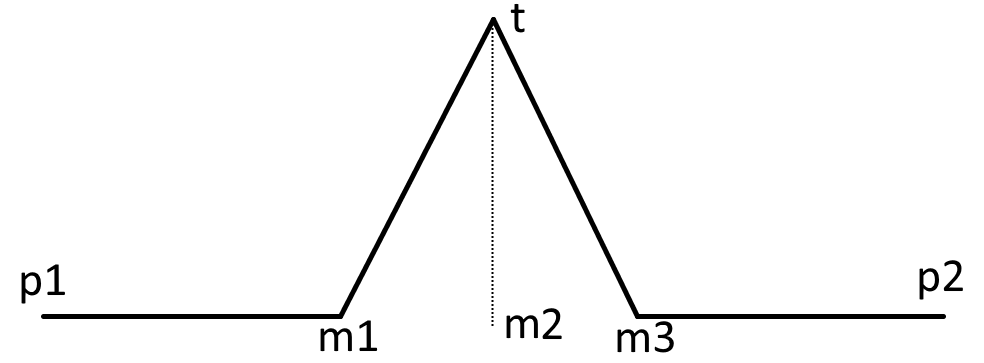
\includegraphics[width=\textwidth]{koch.png}
	\caption{Koch's Curve generatie 1}
	\label{fig:koch}
\end{figure}
\begin{figure}[H]
	\centering
	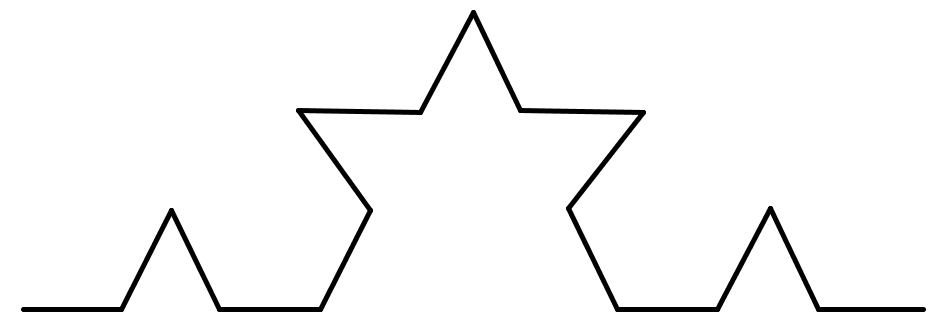
\includegraphics[width=\textwidth]{koch2.png}
	\caption{Koch's Curve generatie 2}
	\label{fig:koch2}
\end{figure}
\begin{figure}[H]
	\centering
	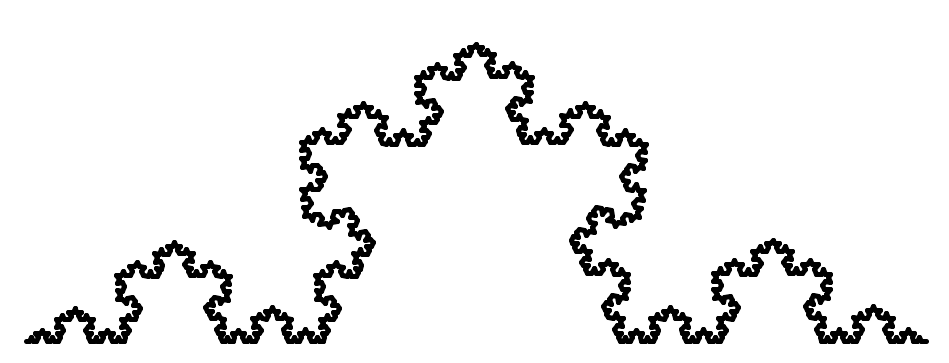
\includegraphics[width=\textwidth]{koch_fract.png}
	\caption{Koch's Curve Fractel (generatie $\infty$)}
	\label{fig:koch_fract}
\end{figure}

In deze opdracht ga je een functie schrijven die dit proces \texttt{n} keer herhaald.\\
Maak gebruik van de al geschreven functie \texttt{kochCurve} van de vorige assignment.
\begin{lstlisting}
void kochCurve(int n,PVector p1, PVector p2) {
    if (n == 0) {
        line(p1.x,p1.y,p2.x,p2.y);
    }else {
        //TODO
    }
}
\end{lstlisting}

\section{[Bonus] Koch's Snowflake}
Door Koch's curve een aantal keer te draaien ontstaat \textbf{Koch's Snowflake}.
\begin{lstlisting}
void kochSnowflake(int n, int sides, int r, PVector center) {
}
\end{lstlisting}
De parameters zijn:
\begin{description}
    \item[n] het aantal itteraties van Koch's curve.
    \item[center] het midden van de snowflake.
    \item[sides] het aantal zijden van de snowflake.
    \item[r] de radius van de snowflake.
\end{description}
\tip{Gebruik de code die je hebt geschreven voor opdracht 2 \texttt{polygon}!}
De volgende code geeft als resultaat figuur \ref{fig:snowflakes}.
\begin{lstlisting}
  snowflake(2,5,50, new PVector(100,200));
  snowflake(5,6,100,new PVector(300,200));
  snowflake(1,6,30, new PVector(500,200));
  snowflake(3,3,100,new PVector(700,200));
\end{lstlisting}
\begin{figure}[H]
	\centering
	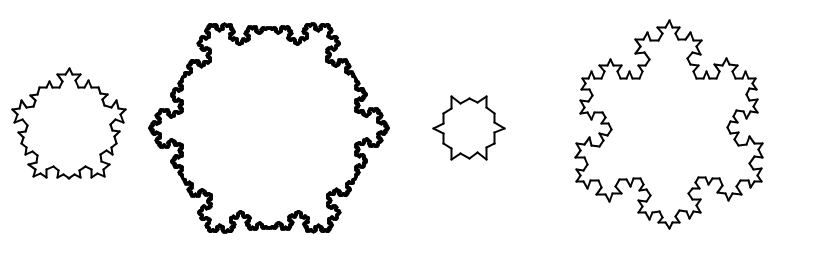
\includegraphics[width=\textwidth]{snowflakes.png}
	\caption{Koch snowflakes!}
	\label{fig:snowflakes}
\end{figure}

\end{document}